\section{Problema 1. Lógica de
predicados}\label{problema-1.-luxf3gica-de-predicados}

\subsection{a) Representación
lógica}\label{a-representaciuxf3n-luxf3gica}

Vocabulario utilizado:

\begin{itemize}
\tightlist
\item
  \texttt{Veterinario(x)}: x es veterinario.
\item
  \texttt{Animal(x)}: x es animal.
\item
  \texttt{AnimalRescatado(x)}: x es animal rescatado.
\item
  \texttt{Atiende(x,\ y)}: x atiende a y.
\item
  \texttt{Vacunado(x)}: x ha recibido una vacuna.
\end{itemize}

\textbf{1. Todos los veterinarios atienden al menos a un animal.}

\begin{verbatim}
∀x (Veterinario(x) → ∃y (Animal(y) ∧ Atiende(x, y)))
\end{verbatim}

Justificación:

\begin{itemize}
\tightlist
\item
  \texttt{∀x} porque es una afirmación universal sobre todos los
  veterinarios.
\item
  Se usa implicación \texttt{→} y no conjunción, porque solo se exige
  algo a quienes cumplen \texttt{Veterinario(x)}.
\item
  \texttt{∃y} porque basta con que exista al menos un animal atendido,
  no todos.
\item
  \texttt{Animal(y)\ ∧\ Atiende(x,\ y)} garantiza que ese individuo sea
  animal y que exista la relación de atención.
\end{itemize}

\textbf{2. Existe al menos un animal rescatado que ha recibido una
vacuna.}

\begin{verbatim}
∃x (AnimalRescatado(x) ∧ Vacunado(x))
\end{verbatim}

Justificación:

\begin{itemize}
\tightlist
\item
  \texttt{∃x} porque basta un caso para que la afirmación sea verdadera.
\item
  Se usa conjunción \texttt{∧} porque el mismo individuo debe cumplir
  ambas propiedades a la vez.
\item
  No se usa implicación, porque no es una regla general sino la
  afirmación de existencia de un individuo con dos características.
\end{itemize}

\subsection{b) Identificación y corrección de
errores}\label{b-identificaciuxf3n-y-correcciuxf3n-de-errores}

Afirmación a representar: \emph{``Todos los animales que reciben una
vacuna son animales rescatados''}.

Expresión propuesta:

\begin{verbatim}
∀x (Vacunado(x) ∧ AnimalRescatado(x))
\end{verbatim}

\textbf{Por qué es incorrecta:}

\begin{enumerate}
\def\labelenumi{\arabic{enumi}.}
\tightlist
\item
  Usa conjunción \texttt{∧} con cuantificador universal. Eso afirma que
  \textbf{todo individuo del universo} cumple ambas cosas a la vez: todo
  es vacunado y todo es animal rescatado.
\item
  No expresa condicionalidad. La frase original es un ``si \ldots{}
  entonces \ldots'': \emph{si} está vacunado, \emph{entonces} es
  rescatado. La fórmula propuesta no tiene \texttt{→} y por tanto no
  restringe, sino que generaliza en exceso.
\item
  Bastaría un contraejemplo (una persona no vacunada, un animal no
  rescatado) para hacer falsa la fórmula, aunque la afirmación original
  podría seguir siendo verdadera.
\end{enumerate}

\textbf{Expresión corregida:}

\begin{verbatim}
∀x (Vacunado(x) → AnimalRescatado(x))
\end{verbatim}

Variante más explícita delimitando a animales:

\begin{verbatim}
∀x ((Animal(x) ∧ Vacunado(x)) → AnimalRescatado(x))
\end{verbatim}

Justificación de la corrección: con \texttt{→} solo se exige
\texttt{AnimalRescatado(x)} a quienes cumplen el antecedente. Los
individuos no vacunados no falsan la fórmula, que es exactamente lo que
pide el enunciado.

\begin{center}\rule{0.5\linewidth}{0.5pt}\end{center}

\section{Problema 2. Diseño de una ontología --- Repositorio
universitario}\label{problema-2.-diseuxf1o-de-una-ontologuxeda-repositorio-universitario}

Dominio: organizar publicaciones para clasificar y consultar; distinguir
digitales e impresas, registrar autores, identificar formatos, reconocer
autoría múltiple y licencia abierta.

\subsection{a) Clases necesarias y
propósito}\label{a-clases-necesarias-y-propuxf3sito}

{\def\LTcaptype{none} % do not increment counter
\begin{longtable}[]{@{}
  >{\raggedright\arraybackslash}p{(\linewidth - 2\tabcolsep) * \real{0.5000}}
  >{\raggedright\arraybackslash}p{(\linewidth - 2\tabcolsep) * \real{0.5000}}@{}}
\toprule\noalign{}
\begin{minipage}[b]{\linewidth}\raggedright
Clase
\end{minipage} & \begin{minipage}[b]{\linewidth}\raggedright
Propósito
\end{minipage} \\
\midrule\noalign{}
\endhead
\bottomrule\noalign{}
\endlastfoot
\texttt{Publicacion} & Clase central. Toda obra del repositorio. \\
\texttt{PublicacionDigital} & Publicaciones en soporte digital. Permite
clasificar y aplicar reglas propias de lo digital. \\
\texttt{PublicacionImpresa} & Publicaciones en soporte físico.
Incompatible con la anterior. \\
\texttt{PublicacionMultiautor} & Clase definida para las publicaciones
con ≥2 autores distintos. Se infiere automáticamente. \\
\texttt{PublicacionDigitalPDF} & Clase definida para publicaciones
digitales disponibles en PDF. Se infiere automáticamente. \\
\texttt{Autor} & Personas que escriben publicaciones. Se vincula vía
\texttt{escritoPor}. \\
\texttt{Formato} & Formatos de disponibilidad. Ej.: \texttt{PDF},
\texttt{EPUB}, \texttt{HTML}, \texttt{TapaBlanda}, \texttt{TapaDura}. \\
\texttt{Licencia} & Licencias de uso de la publicación. \\
\texttt{LicenciaAbierta} & Subclase de \texttt{Licencia} para acceso
abierto (ej. Creative Commons). Permite filtrar qué se puede difundir
libremente. \\
\end{longtable}
}

Individuos ejemplo (a usar en Protégé, Problema 4): \texttt{pub1},
\texttt{pub2}, \texttt{autor1}, \texttt{autor2}, \texttt{formatoPDF}.

\subsection{b) Relaciones entre
conceptos}\label{b-relaciones-entre-conceptos}

{\def\LTcaptype{none} % do not increment counter
\begin{longtable}[]{@{}
  >{\raggedright\arraybackslash}p{(\linewidth - 2\tabcolsep) * \real{0.5000}}
  >{\raggedright\arraybackslash}p{(\linewidth - 2\tabcolsep) * \real{0.5000}}@{}}
\toprule\noalign{}
\begin{minipage}[b]{\linewidth}\raggedright
Propiedad (dominio → rango)
\end{minipage} & \begin{minipage}[b]{\linewidth}\raggedright
Qué información representa
\end{minipage} \\
\midrule\noalign{}
\endhead
\bottomrule\noalign{}
\endlastfoot
\texttt{escritoPor} (\texttt{Publicacion\ →\ Autor}) & Autoría. Quién
escribió cada publicación. Base para \texttt{PublicacionMultiautor}.
Inversa: \texttt{esAutorDe}. \\
\texttt{disponibleEn} (\texttt{Publicacion\ →\ Formato}) & En qué
formato(s) está disponible cada publicación. Base para
\texttt{PublicacionDigitalPDF}. \\
\texttt{tieneLicencia} (\texttt{Publicacion\ →\ Licencia}) & Bajo qué
licencia se publica. Permite identificar licencia abierta. \\
\end{longtable}
}

Se modelan como \texttt{ObjectProperty}, no como cadenas de texto, para
poder razonar sobre los individuos relacionados y mantener integridad
referencial.

\subsection{c) Jerarquía de clases y
restricciones}\label{c-jerarquuxeda-de-clases-y-restricciones}

Representación textual:

\begin{verbatim}
Publicacion
  ├─ PublicacionDigital
  ├─ PublicacionImpresa
  ├─ PublicacionMultiautor      [definida]
  └─ PublicacionDigitalPDF      [definida]

Autor
Formato
  ├─ (individuos: PDF, EPUB, HTML, TapaBlanda, ...)
Licencia
  └─ LicenciaAbierta
\end{verbatim}

Restricciones (Manchester):

\begin{verbatim}
1. PublicacionDigital SubClassOf Publicacion
2. PublicacionImpresa SubClassOf Publicacion
3. PublicacionDigital DisjointWith PublicacionImpresa
4. PublicacionMultiautor EquivalentTo Publicacion and (escritoPor min 2 Autor)
5. PublicacionDigitalPDF EquivalentTo PublicacionDigital and (disponibleEn value PDF)
   // alternativa con clase: ... and (disponibleEn some FormatoPDF)
6. Publicacion SubClassOf (escritoPor some Autor)
7. Publicacion SubClassOf (disponibleEn some Formato)
8. LicenciaAbierta SubClassOf Licencia
9. PublicacionConLicenciaAbierta EquivalentTo Publicacion and (tieneLicencia some LicenciaAbierta)
\end{verbatim}

Coherencia que aportan:

\begin{itemize}
\tightlist
\item
  1-3 garantizan la distinción digital/impreso y la incompatibilidad
  exigida en el Problema 4.
\item
  4-5 son clases definidas (\texttt{EquivalentTo}), permiten
  clasificación automática por HermiT.
\item
  6-7 evitan publicaciones sin autor ni formato.
\item
  9 permite consultar qué se puede difundir en abierto.
\end{itemize}

\subsection{d) Justificación de dos decisiones de
diseño}\label{d-justificaciuxf3n-de-dos-decisiones-de-diseuxf1o}

\textbf{Decisión 1: \texttt{Formato} como clase con individuos
(\texttt{PDF}, \ldots) y no como \texttt{xsd:string}.} Si
\texttt{formato} fuera un dato literal (\texttt{titulo},
\texttt{"PDF"}), no se podría usar \texttt{disponibleEn\ value\ PDF} ni
\texttt{some\ FormatoPDF} para definir \texttt{PublicacionDigitalPDF},
ni distinguir formatos digitales de impresos con jerarquía. Con clase,
el razonador puede inferir y se puede extender (nuevo formato = nuevo
individuo, sin cambiar el esquema).

\textbf{Decisión 2: \texttt{PublicacionMultiautor} y
\texttt{PublicacionDigitalPDF} como clases definidas
(\texttt{EquivalentTo}) y no como subclases primitivas
(\texttt{SubClassOf}).} Si fueran primitivas, habría que clasificar
manualmente cada individuo y se podría olvidar o equivocar. Como
definidas (condición necesaria y suficiente), HermiT clasifica solo
cuando se cumplen \texttt{min\ 2} autores o \texttt{Digital\ +\ PDF}.
Sin \texttt{EquivalentTo} no habría inferencia automática, que es justo
lo que piden los requisitos funcionales del Problema 4.

\begin{center}\rule{0.5\linewidth}{0.5pt}\end{center}

\section{Problema 3. Interpretación de axiomas
OWL}\label{problema-3.-interpretaciuxf3n-de-axiomas-owl}

\subsection{a) Subclases}\label{a-subclases}

\begin{verbatim}
PublicacionDigital SubClassOf Publicacion
\end{verbatim}

Significa que todo individuo de \texttt{PublicacionDigital} es también
individuo de \texttt{Publicacion}. Es inclusión de conjuntos, no
igualdad: puede haber publicaciones que no sean digitales (las
impresas). La subclase hereda las restricciones de la superclase: si
\texttt{Publicacion} exige \texttt{escritoPor\ some\ Autor}, toda
digital también debe cumplirlo.

\subsection{\texorpdfstring{b) Restricciones \texttt{some} vs
\texttt{only}}{b) Restricciones some vs only}}\label{b-restricciones-some-vs-only}

\begin{itemize}
\item
  \texttt{escritoPor\ some\ Autor} (existencial /
  \texttt{someValuesFrom}): Garantiza que \textbf{existe al menos un}
  valor de \texttt{escritoPor} que es \texttt{Autor}. No garantiza que
  \emph{todos} lo sean, ni cuántos hay. Una publicación con un autor
  válido y otros valores no-autor seguiría cumpliéndola.
\item
  \texttt{escritoPor\ only\ Autor} (universal / \texttt{allValuesFrom}):
  Garantiza que \textbf{todos} los valores de \texttt{escritoPor}, si
  existen, son de tipo \texttt{Autor}. No garantiza existencia: si la
  publicación no tiene ningún \texttt{escritoPor}, la restricción se
  cumple por vacío (verdad vacuosa).
\end{itemize}

En la práctica se combinan: \texttt{escritoPor\ some\ Autor} para exigir
autor, \texttt{escritoPor\ only\ Autor} para prohibir valores no-autor.

\subsection{c) Cardinalidad}\label{c-cardinalidad}

\textbf{1. Definición OWL adecuada (Manchester):}

\begin{verbatim}
Class: PublicacionMultiautor
  EquivalentTo: Publicacion and (escritoPor min 2 Autor)
\end{verbatim}

Se usa \texttt{EquivalentTo} (no solo \texttt{SubClassOf}) para que el
razonador infiera automáticamente la pertenencia cuando se cumple el
mínimo. \texttt{min\ 2} exige al menos dos valores distintos en
\texttt{Autor}.

\textbf{2. Por qué dos nombres no bastan:}

OWL \textbf{no asume nombre único (UNA)}. Dos IRI distintos
(\texttt{autor1}, \texttt{autor2}) pueden denotar al mismo individuo
salvo que se declare lo contrario. El razonador puede fusionarlos y
contar 1 solo autor.

Para que cuenten como 2 se debe declarar:

\begin{verbatim}
DifferentIndividuals: autor1, autor2
\end{verbatim}

o bien:

\begin{verbatim}
autor1 DifferentFrom autor2
\end{verbatim}

Sin esto, \texttt{escritoPor\ min\ 2} podría no dispararse aunque se
hayan registrado dos nombres.

\subsection{d) Equivalencia de clases}\label{d-equivalencia-de-clases}

\texttt{EquivalentTo} define condición \textbf{necesaria y suficiente}.
No solo dice ``todo miembro cumple esto'' (como \texttt{SubClassOf}),
sino también ``todo lo que cumple esto es miembro''. Eso permite al
razonador \textbf{clasificar automáticamente} individuos que no fueron
tipados explícitamente.

Ejemplo del repositorio:

\begin{verbatim}
Class: PublicacionDigitalPDF
  EquivalentTo: PublicacionDigital and (disponibleEn value PDF)
\end{verbatim}

Si se registra \texttt{pub1\ type\ PublicacionDigital} +
\texttt{pub1\ disponibleEn\ PDF}, sin decir que es
\texttt{PublicacionDigitalPDF}, HermiT lo infiere como miembro. Con solo
\texttt{SubClassOf} esa inferencia no ocurriría.

\begin{center}\rule{0.5\linewidth}{0.5pt}\end{center}

\section{Problema 4. Construcción y razonamiento en
Protégé}\label{problema-4.-construcciuxf3n-y-razonamiento-en-protuxe9guxe9}

Ontología construida desde cero en Protégé. IRI:
\texttt{http://www.semanticweb.org/user/ontologies/2026/9/untitled-ontology-5}.
Archivo de entrega: \texttt{Roger.owl} (mismo modelo del Problema 2).

\subsection{a) Modelo construido e individuos
registrados}\label{a-modelo-construido-e-individuos-registrados}

Creación de las 4 subclases del caso en pestaña Entities/clasess

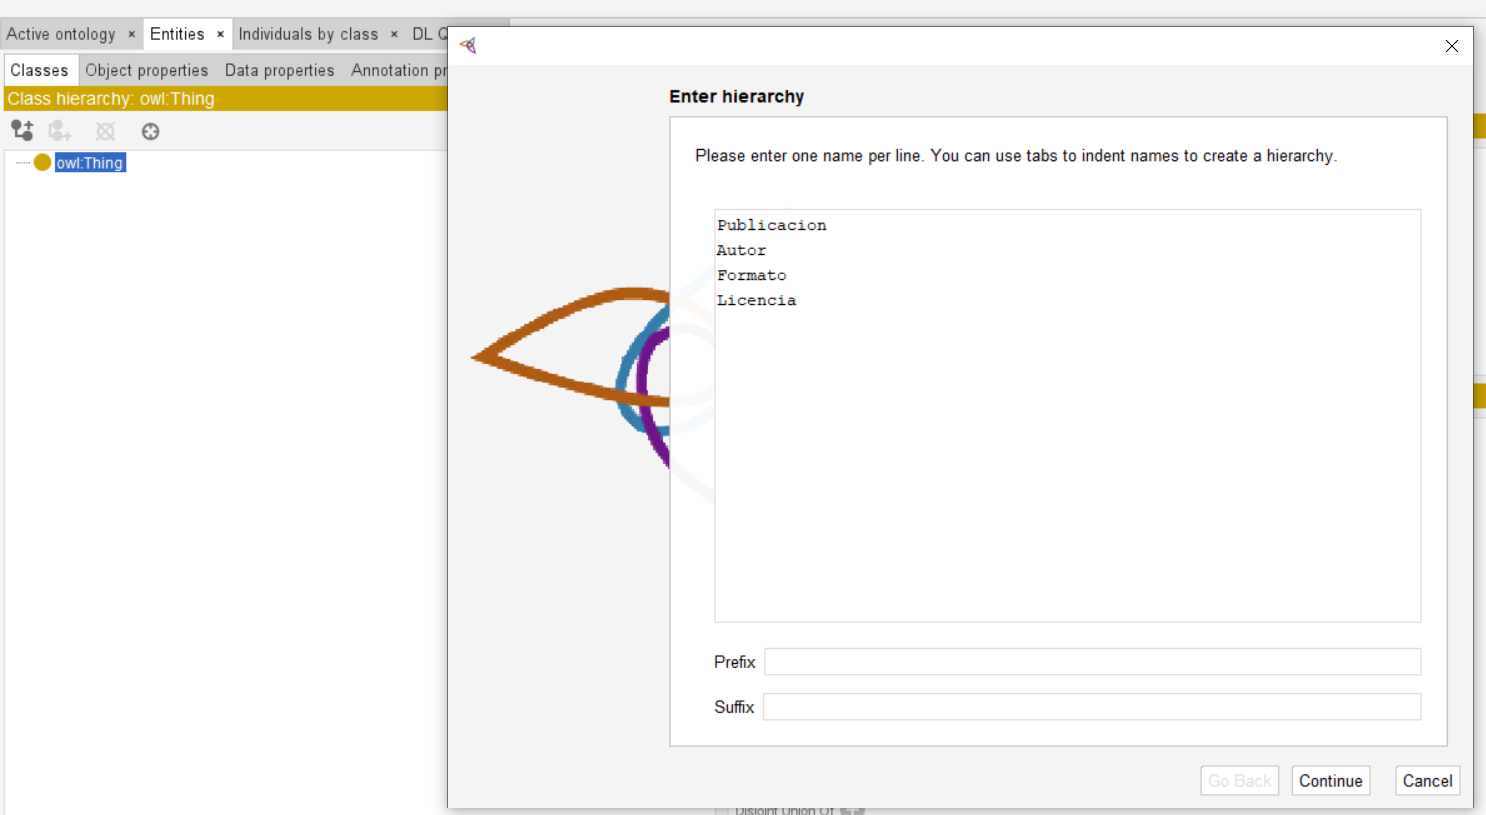
\includegraphics[width=0.86\linewidth,height=\textheight,keepaspectratio]{capturas/p4_01.png}\}

Evidencia de las subclases

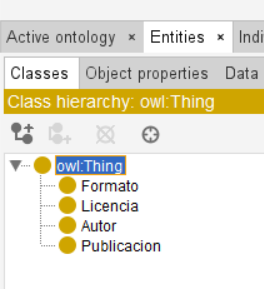
\includegraphics[width=0.45\linewidth,height=\textheight,keepaspectratio]{capturas/p4_02.png}\}

Creación de las subclases de Publicacion, Licencia y publicaciónDigital
para terminar de conformar la jerarquía de clases

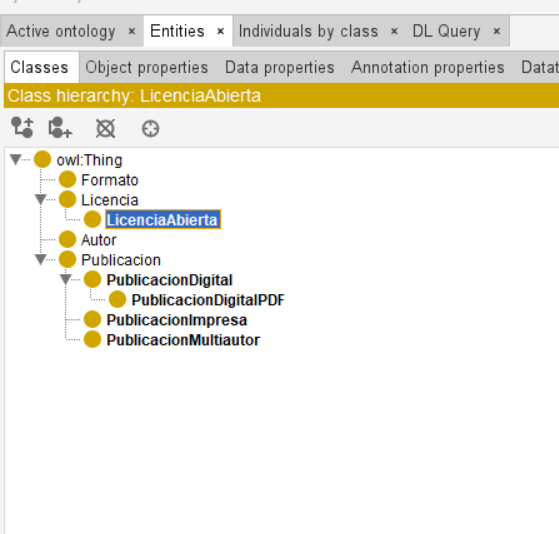
\includegraphics[width=0.86\linewidth,height=\textheight,keepaspectratio]{capturas/p4_03.png}\}

Configuración de la disjunción en PublicacionDigital

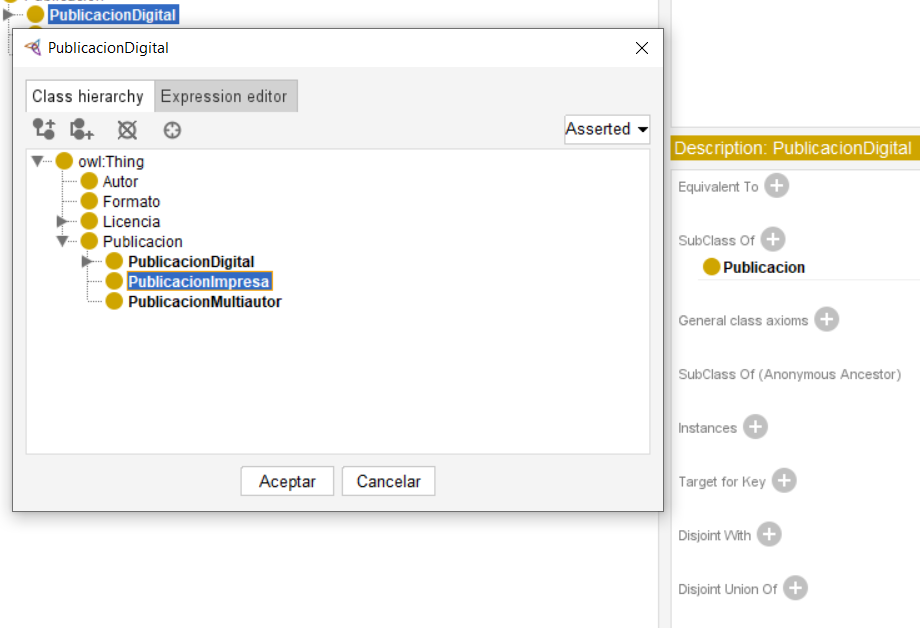
\includegraphics[width=0.86\linewidth,height=\textheight,keepaspectratio]{capturas/p4_04.png}\}

Creación de las propiedades en pestañas object properties y data
properties:

Nos situamos en la pestaña Entities/object properties

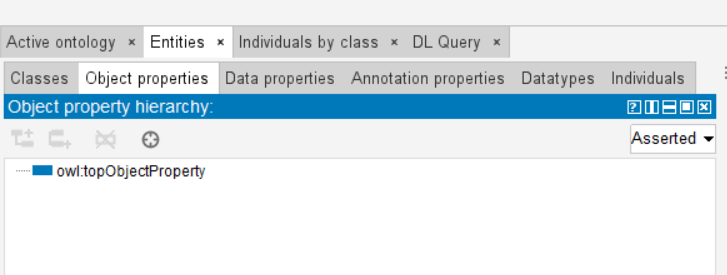
\includegraphics[width=0.86\linewidth,height=\textheight,keepaspectratio]{capturas/p4_05.png}\}

Y creamos 3 propiedades donde posteriormente pasaremos a configurar el
dominio y rango

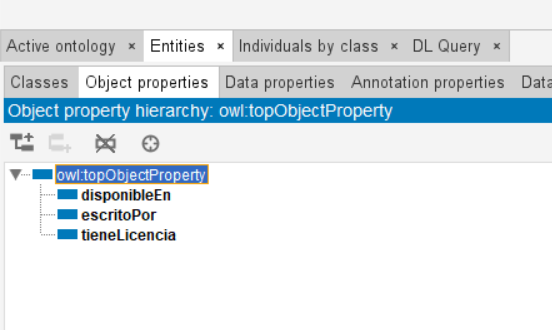
\includegraphics[width=0.86\linewidth,height=\textheight,keepaspectratio]{capturas/p4_06.png}\}

Mostrando la configuración de dominio y rango

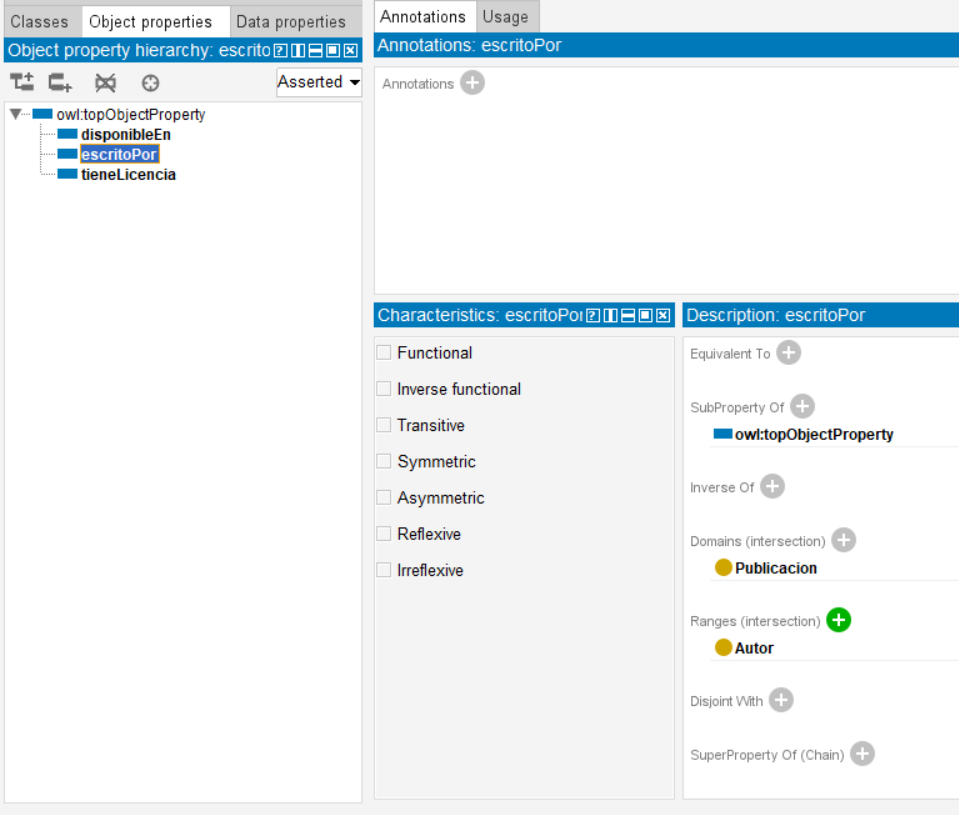
\includegraphics[width=0.86\linewidth,height=\textheight,keepaspectratio]{capturas/p4_07.png}\}

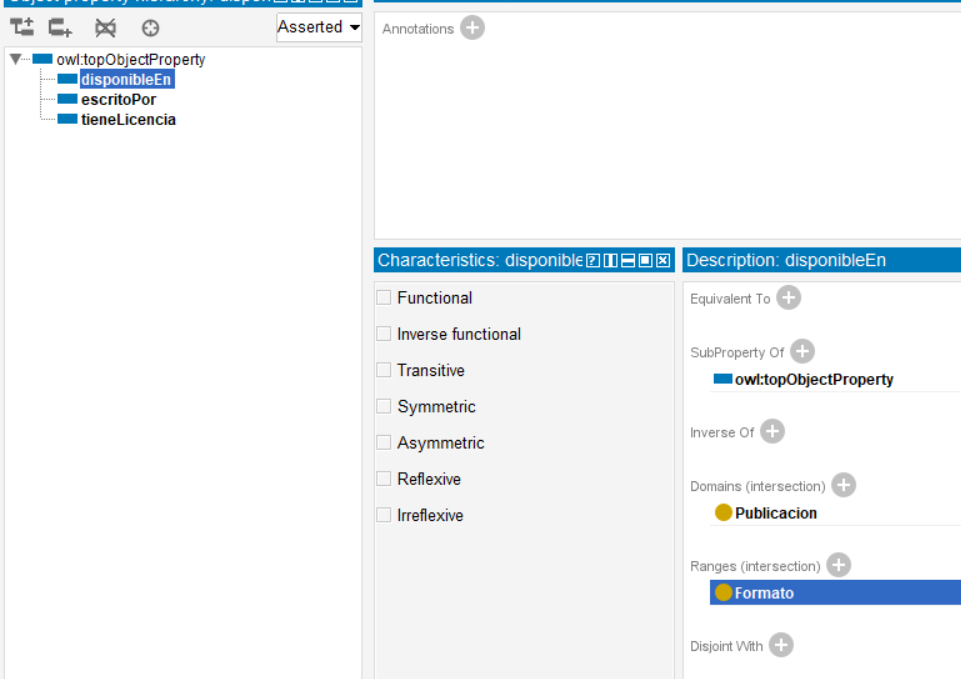
\includegraphics[width=0.86\linewidth,height=\textheight,keepaspectratio]{capturas/p4_08.png}\}

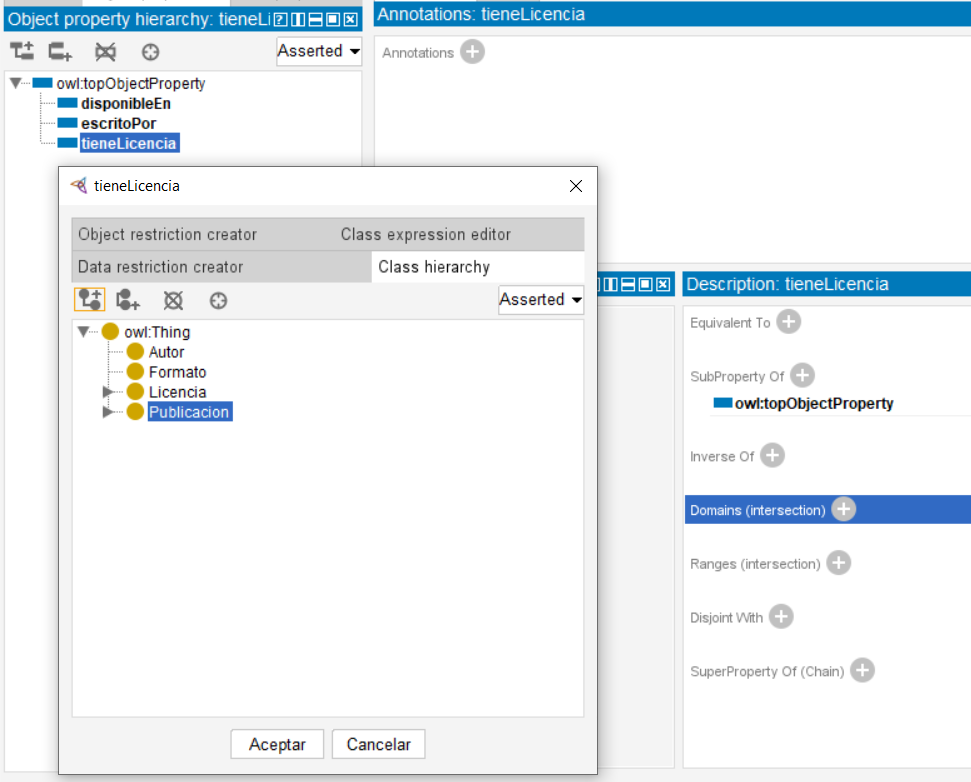
\includegraphics[width=0.86\linewidth,height=\textheight,keepaspectratio]{capturas/p4_09.png}\}

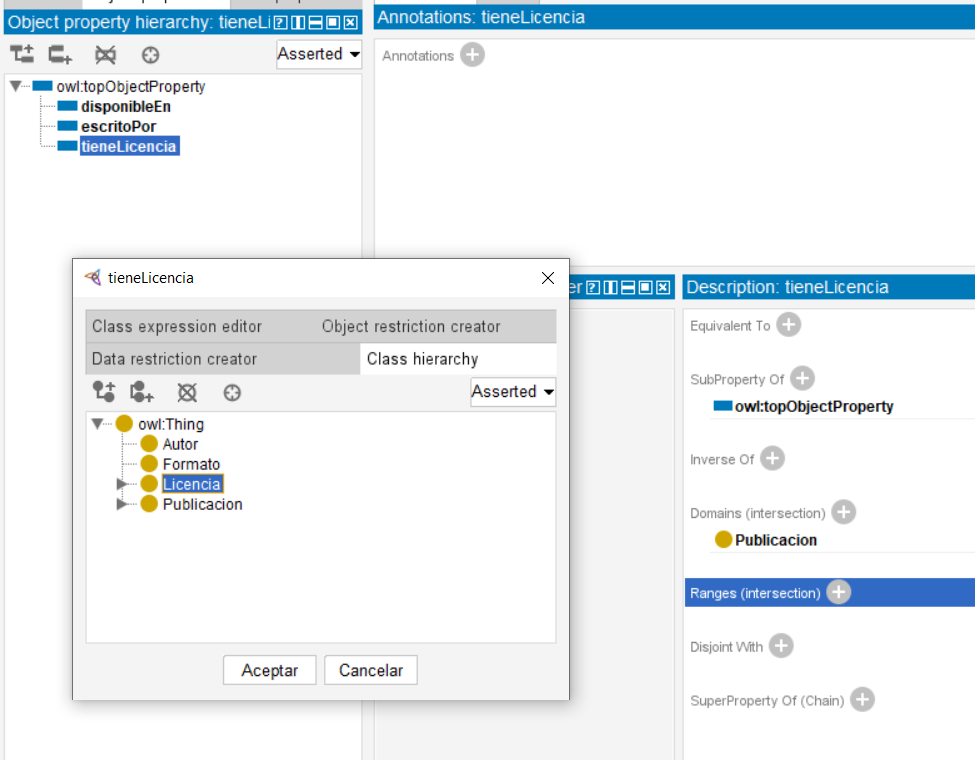
\includegraphics[width=0.86\linewidth,height=\textheight,keepaspectratio]{capturas/p4_10.png}\}

Ahora en Data properties

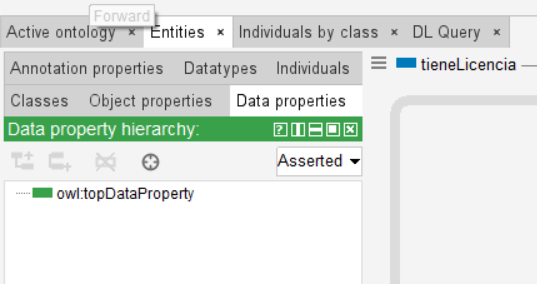
\includegraphics[width=0.82\linewidth,height=\textheight,keepaspectratio]{capturas/p4_11.png}\}

Creamos la propiedad titulo configurando su dominio y rango

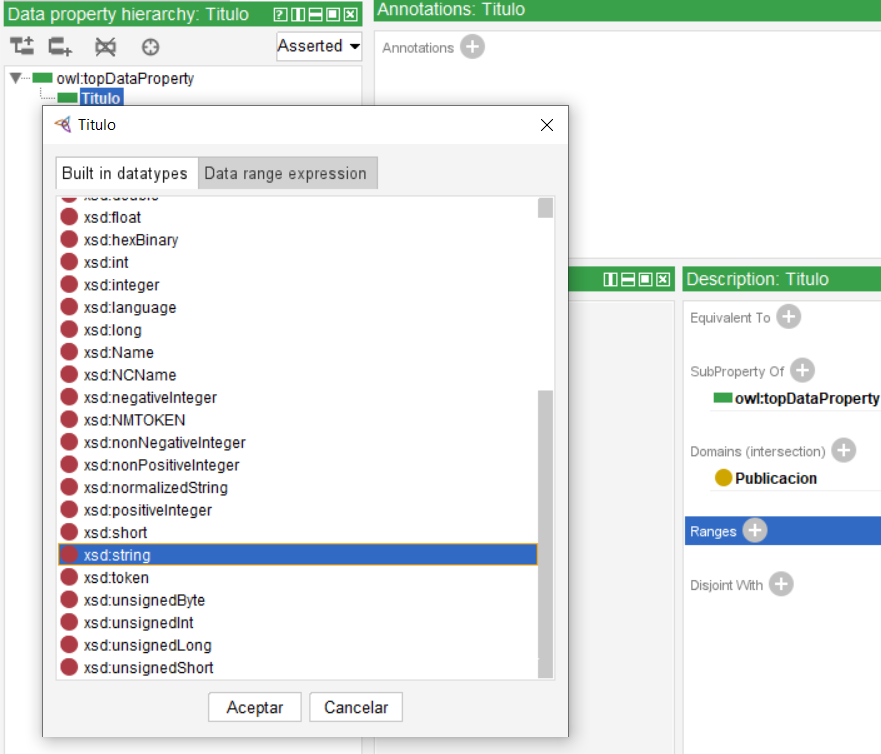
\includegraphics[width=0.86\linewidth,height=\textheight,keepaspectratio]{capturas/p4_12.png}\}

Seguidamente iremos a la pestaña Individuals by class para crear los
individuos de apoyo y diferenciarlos

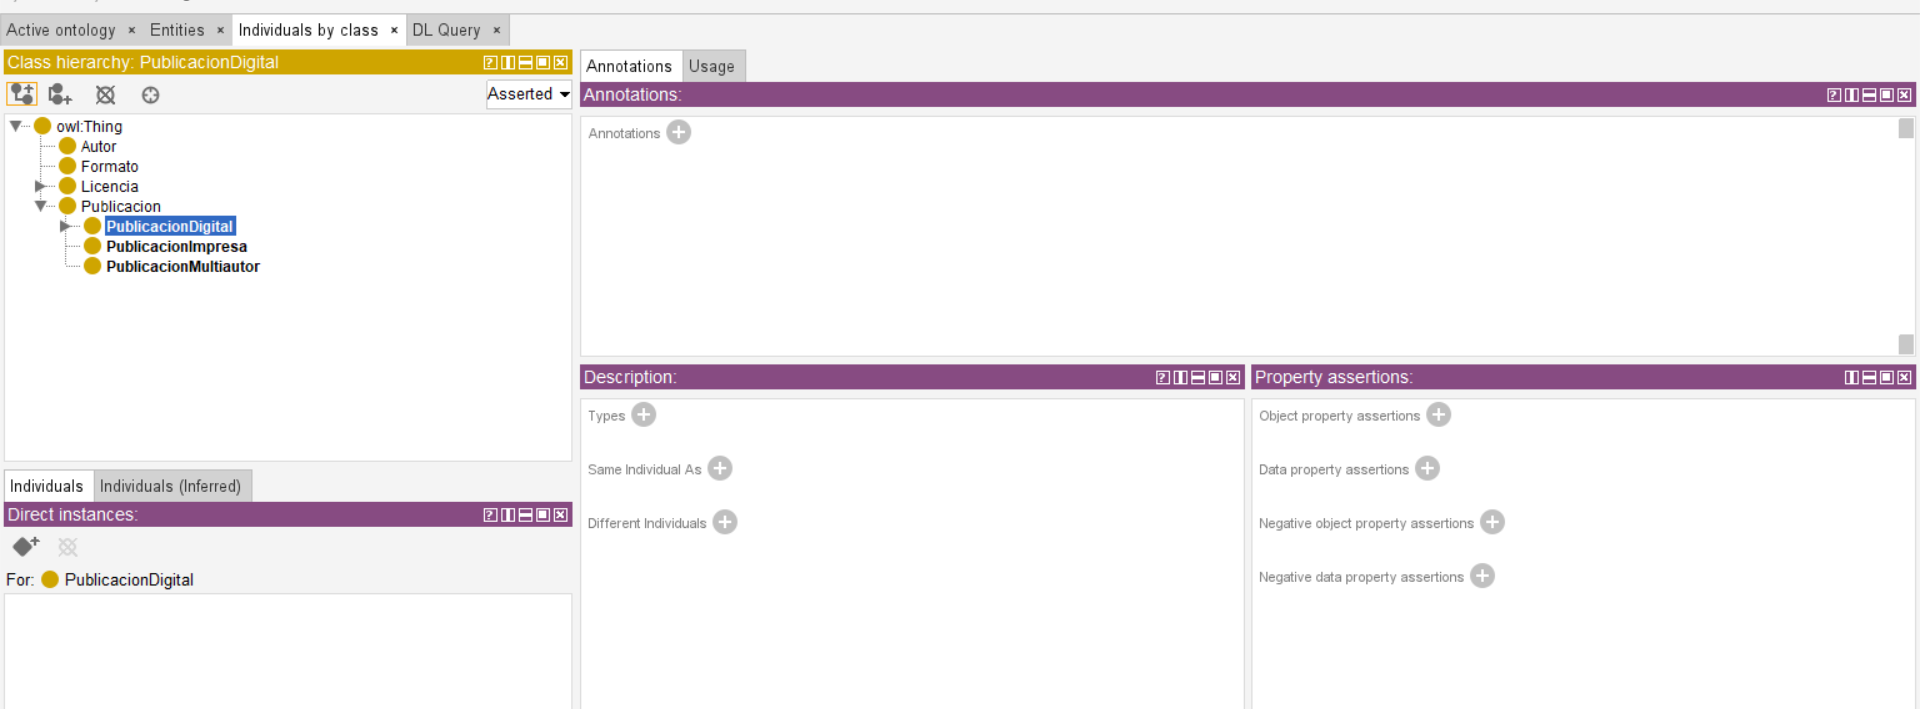
\includegraphics[width=0.86\linewidth,height=\textheight,keepaspectratio]{capturas/p4_13.png}\}

Iniciando con la creación de 3 individuos para la subclase Formato, la
creación es presionando el rombo gris con un + arriba a la derecha

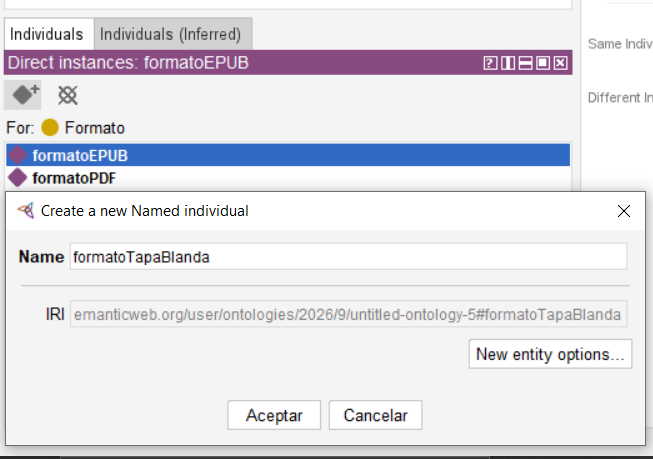
\includegraphics[width=0.86\linewidth,height=\textheight,keepaspectratio]{capturas/p4_14.png}\}

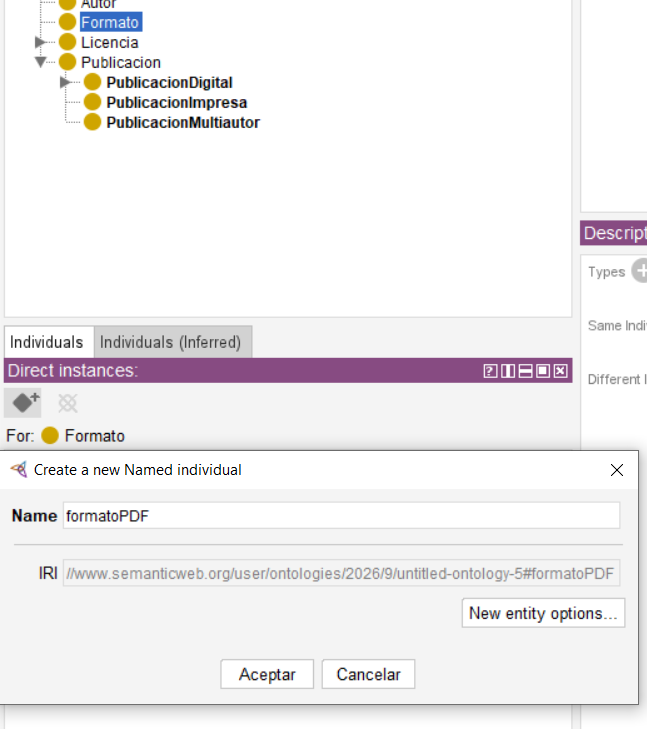
\includegraphics[width=0.86\linewidth,height=\textheight,keepaspectratio]{capturas/p4_15.png}\}

Lo mismo para Licencia

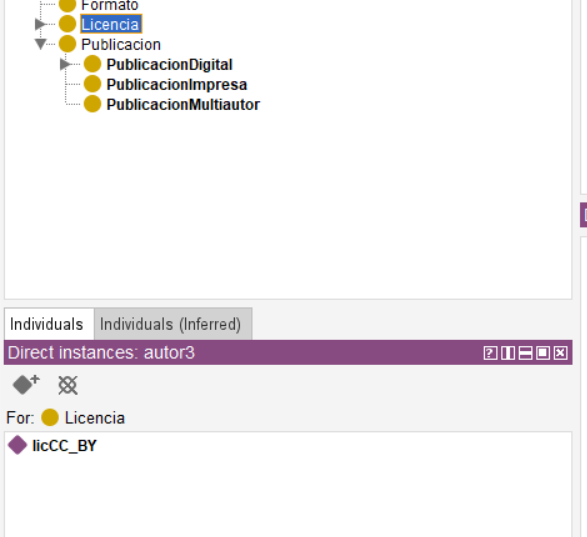
\includegraphics[width=0.86\linewidth,height=\textheight,keepaspectratio]{capturas/p4_16.png}\}

Y para Autor con sus 3 autores y marcando en este punto una
diferenciación

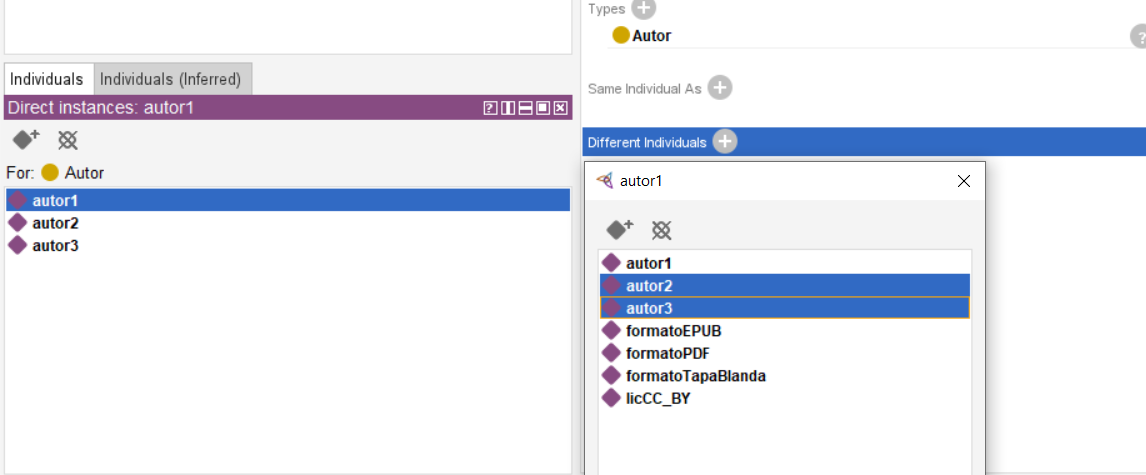
\includegraphics[width=0.86\linewidth,height=\textheight,keepaspectratio]{capturas/p4_17.png}\}

Pasamos a configurar las reglas lógicas de equivalencia {[}Equivalent
to{]} para PublicacionMultiautor y PublicacionDigitalPDF

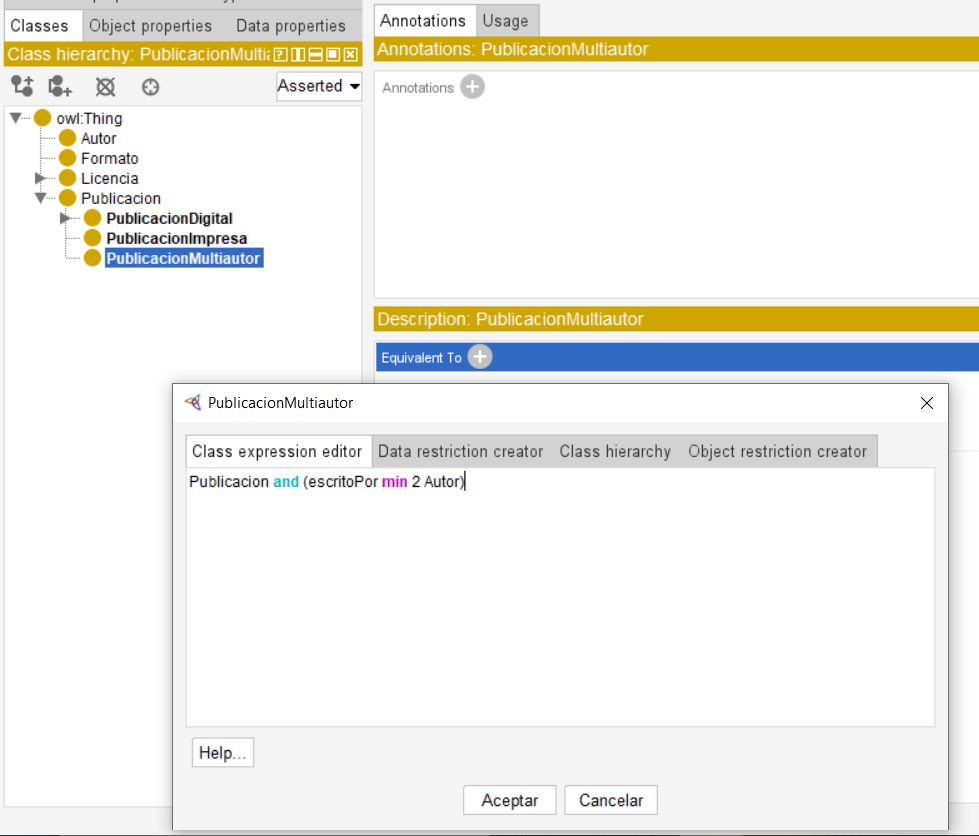
\includegraphics[width=0.86\linewidth,height=\textheight,keepaspectratio]{capturas/p4_18.png}\}

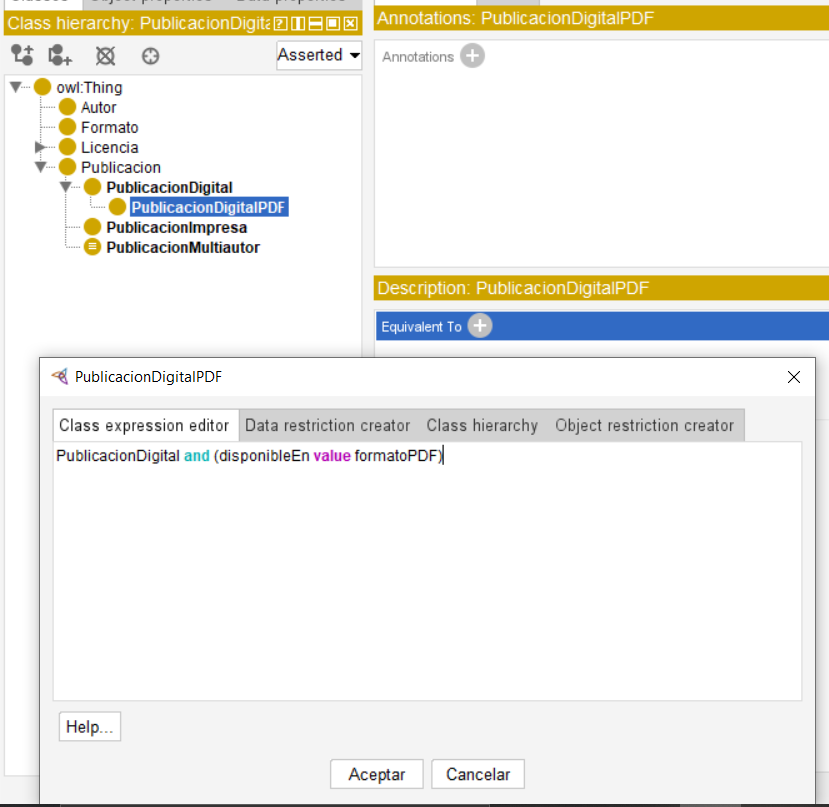
\includegraphics[width=0.86\linewidth,height=\textheight,keepaspectratio]{capturas/p4_19.png}\}

Continuamos con las publicaciones de prueba

pub1\_TesisIA

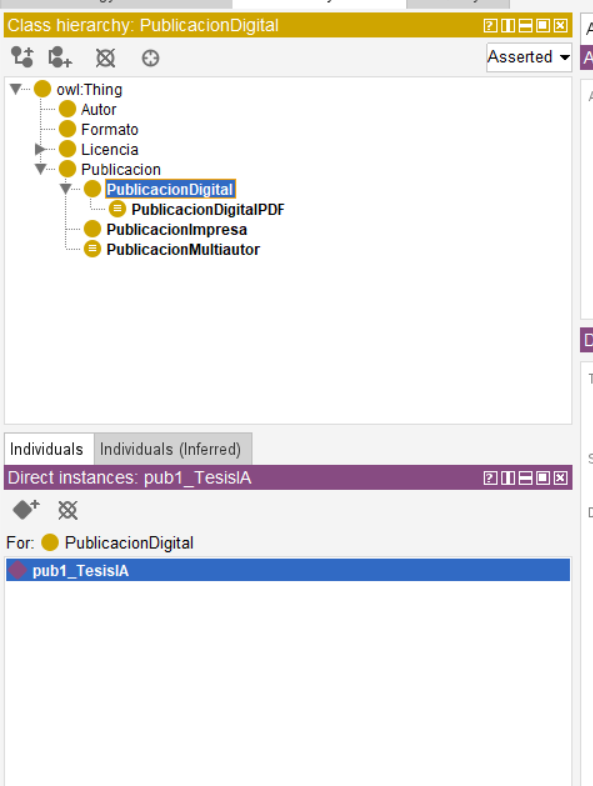
\includegraphics[width=0.86\linewidth,height=\textheight,keepaspectratio]{capturas/p4_20.png}\}

Y asignamos las relaciones {[}Object property assertions{]} y título
{[}Data property assertions{]}

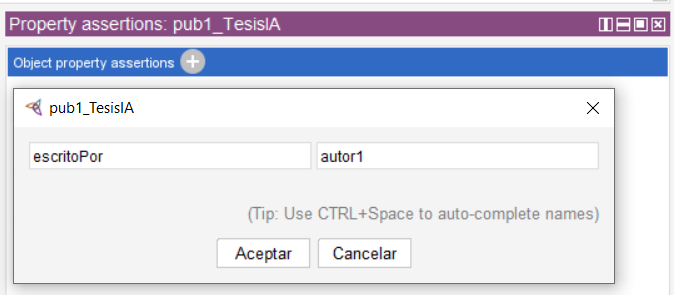
\includegraphics[width=0.86\linewidth,height=\textheight,keepaspectratio]{capturas/p4_21.png}\}

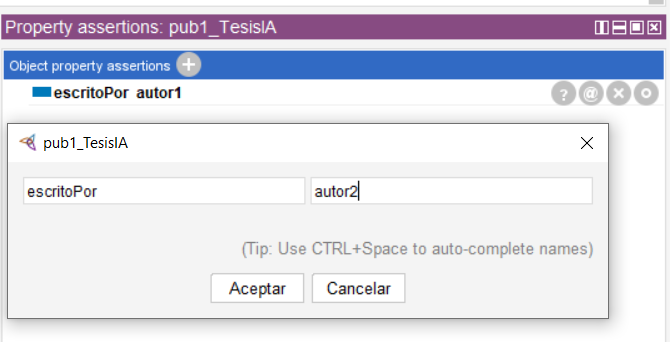
\includegraphics[width=0.86\linewidth,height=\textheight,keepaspectratio]{capturas/p4_22.png}\}

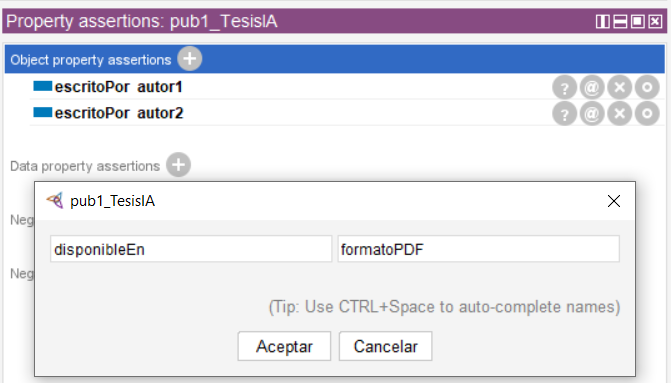
\includegraphics[width=0.86\linewidth,height=\textheight,keepaspectratio]{capturas/p4_23.png}\}

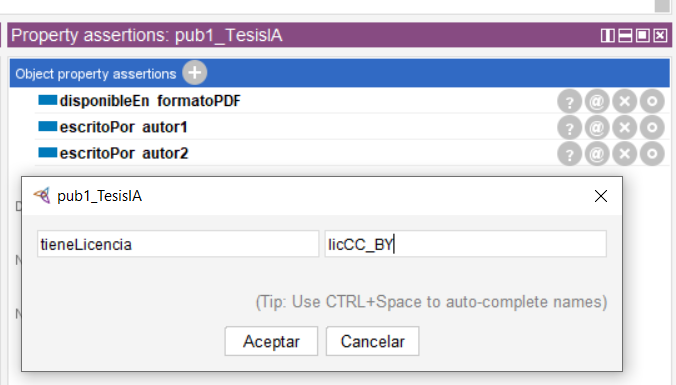
\includegraphics[width=0.86\linewidth,height=\textheight,keepaspectratio]{capturas/p4_24.png}\}

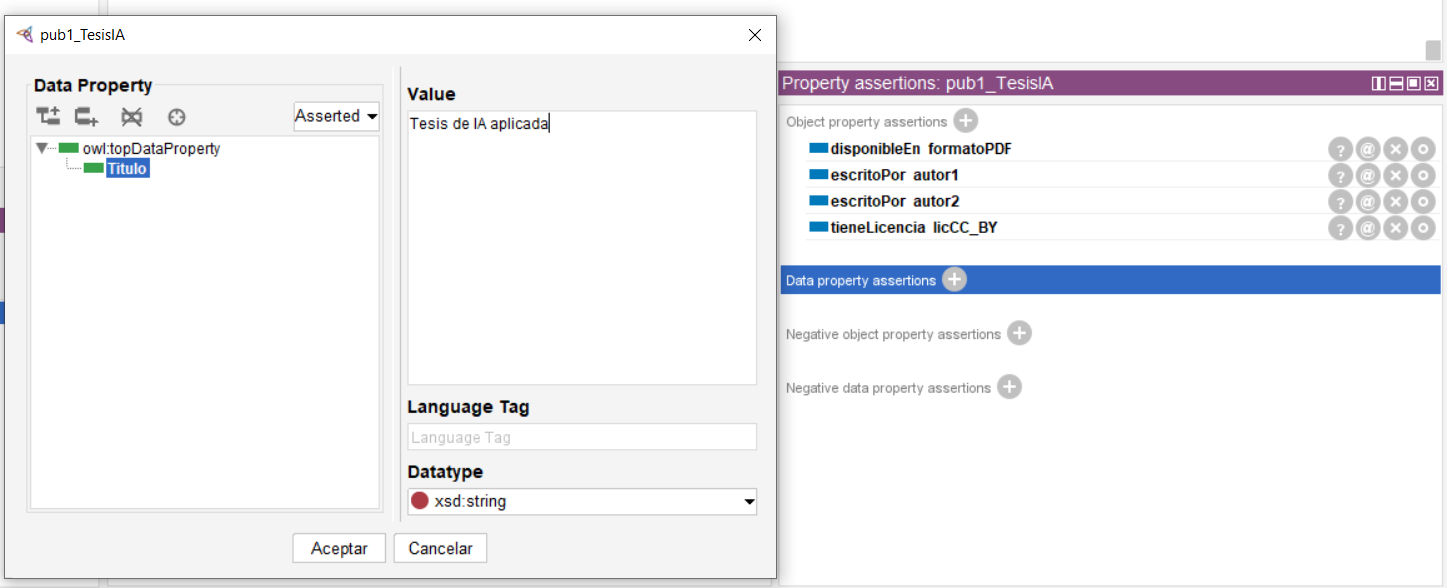
\includegraphics[width=0.86\linewidth,height=\textheight,keepaspectratio]{capturas/p4_25.png}\}

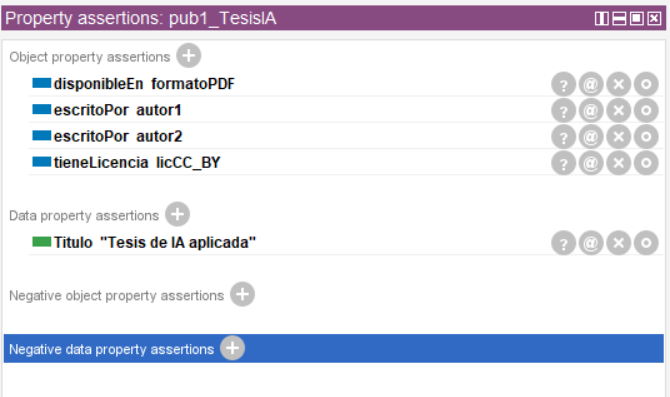
\includegraphics[width=0.86\linewidth,height=\textheight,keepaspectratio]{capturas/p4_26.png}\}
Una vez finalizado probamos la ejecución en el modelo Hermit

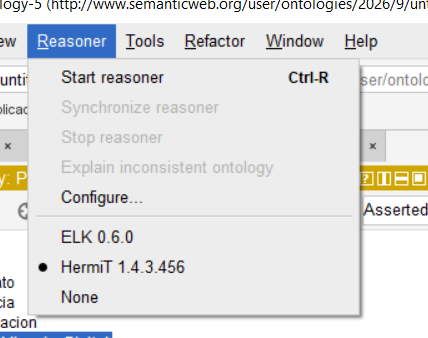
\includegraphics[width=0.65\linewidth,height=\textheight,keepaspectratio]{capturas/p4_27.png}\}

Inciso c

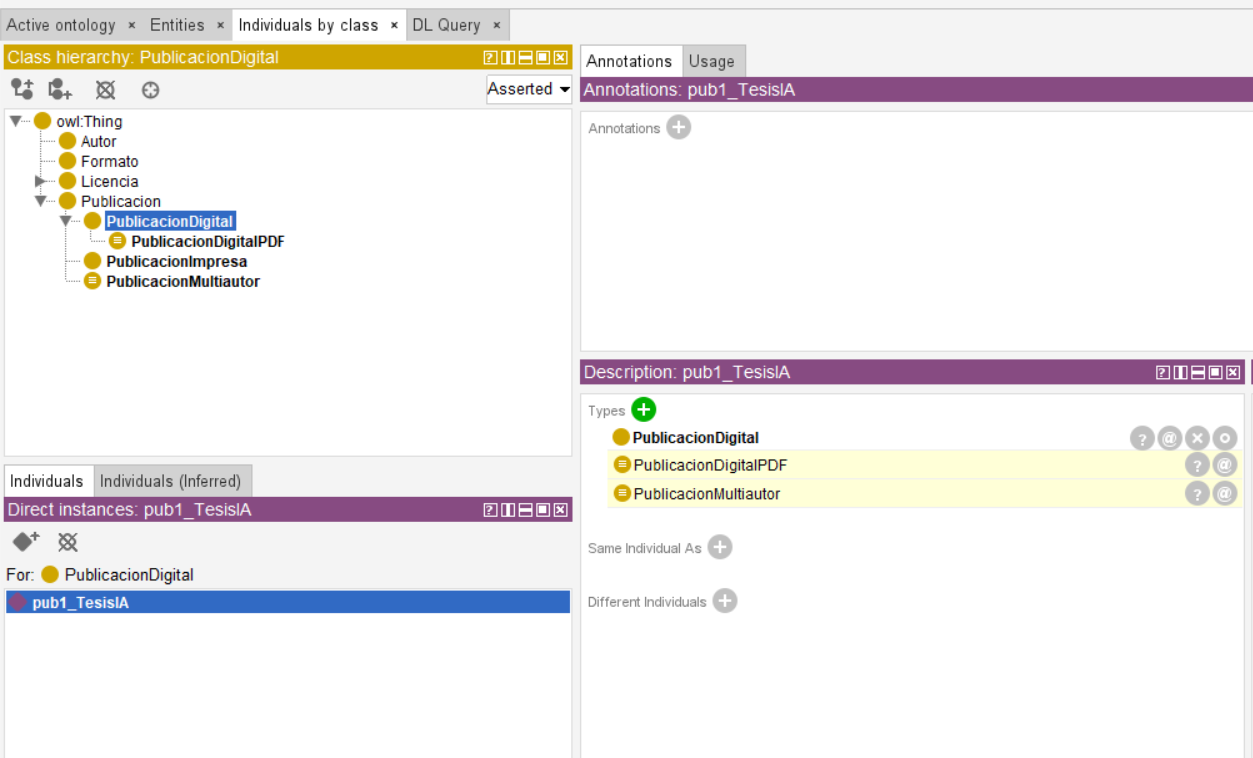
\includegraphics[width=0.86\linewidth,height=\textheight,keepaspectratio]{capturas/p4_28.png}\}

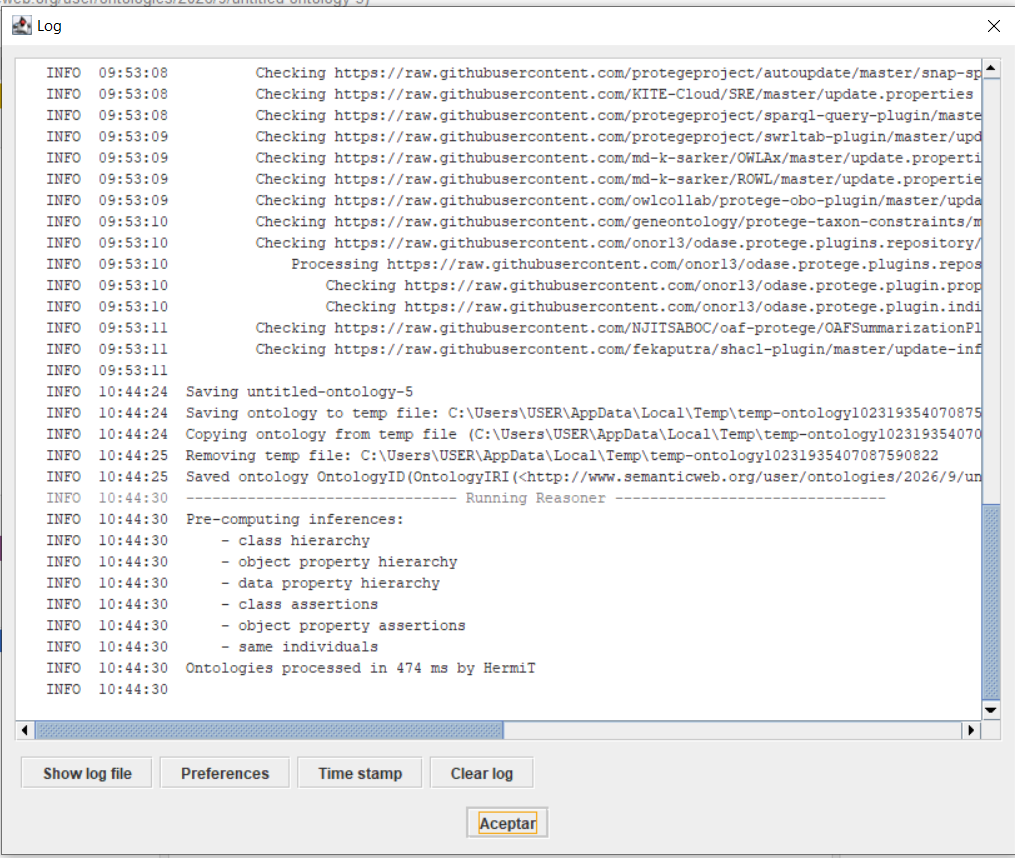
\includegraphics[width=0.86\linewidth,height=\textheight,keepaspectratio]{capturas/p4_29.png}\}

Inciso d

Comprobando el error añadiendo PublicacionImpresa

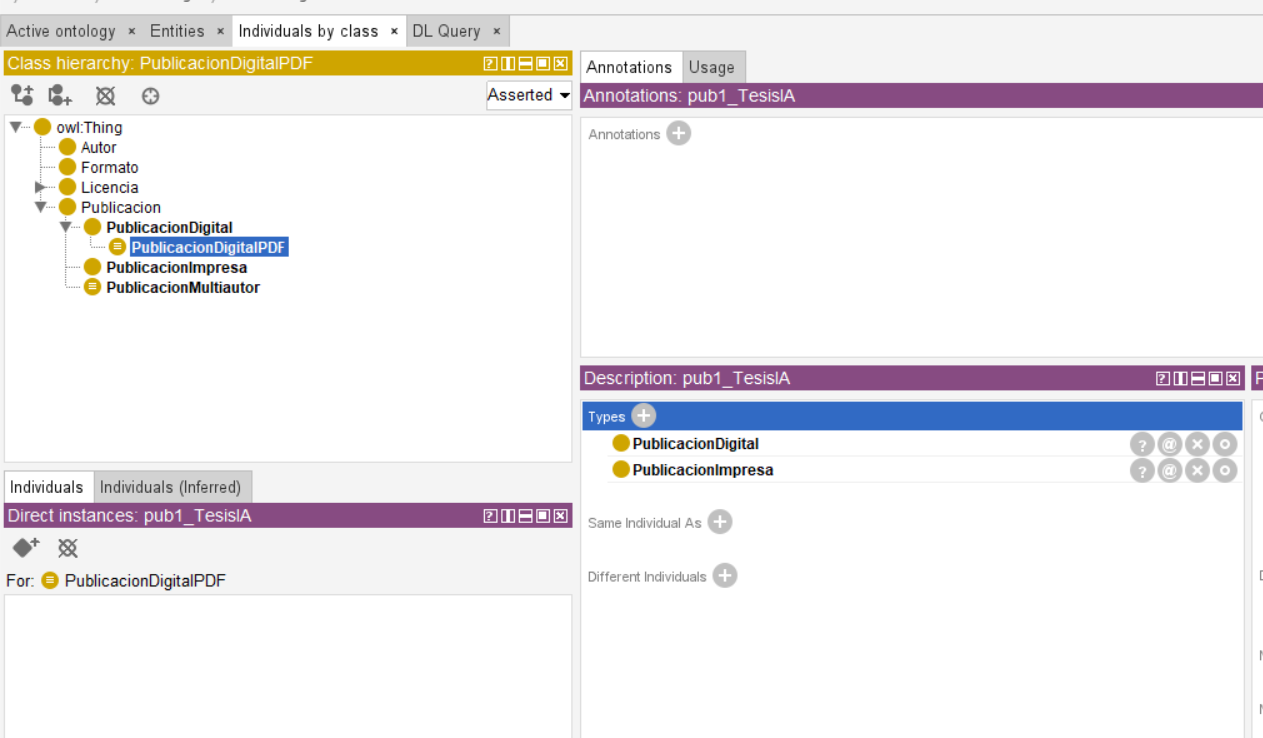
\includegraphics[width=0.86\linewidth,height=\textheight,keepaspectratio]{capturas/p4_30.png}\}

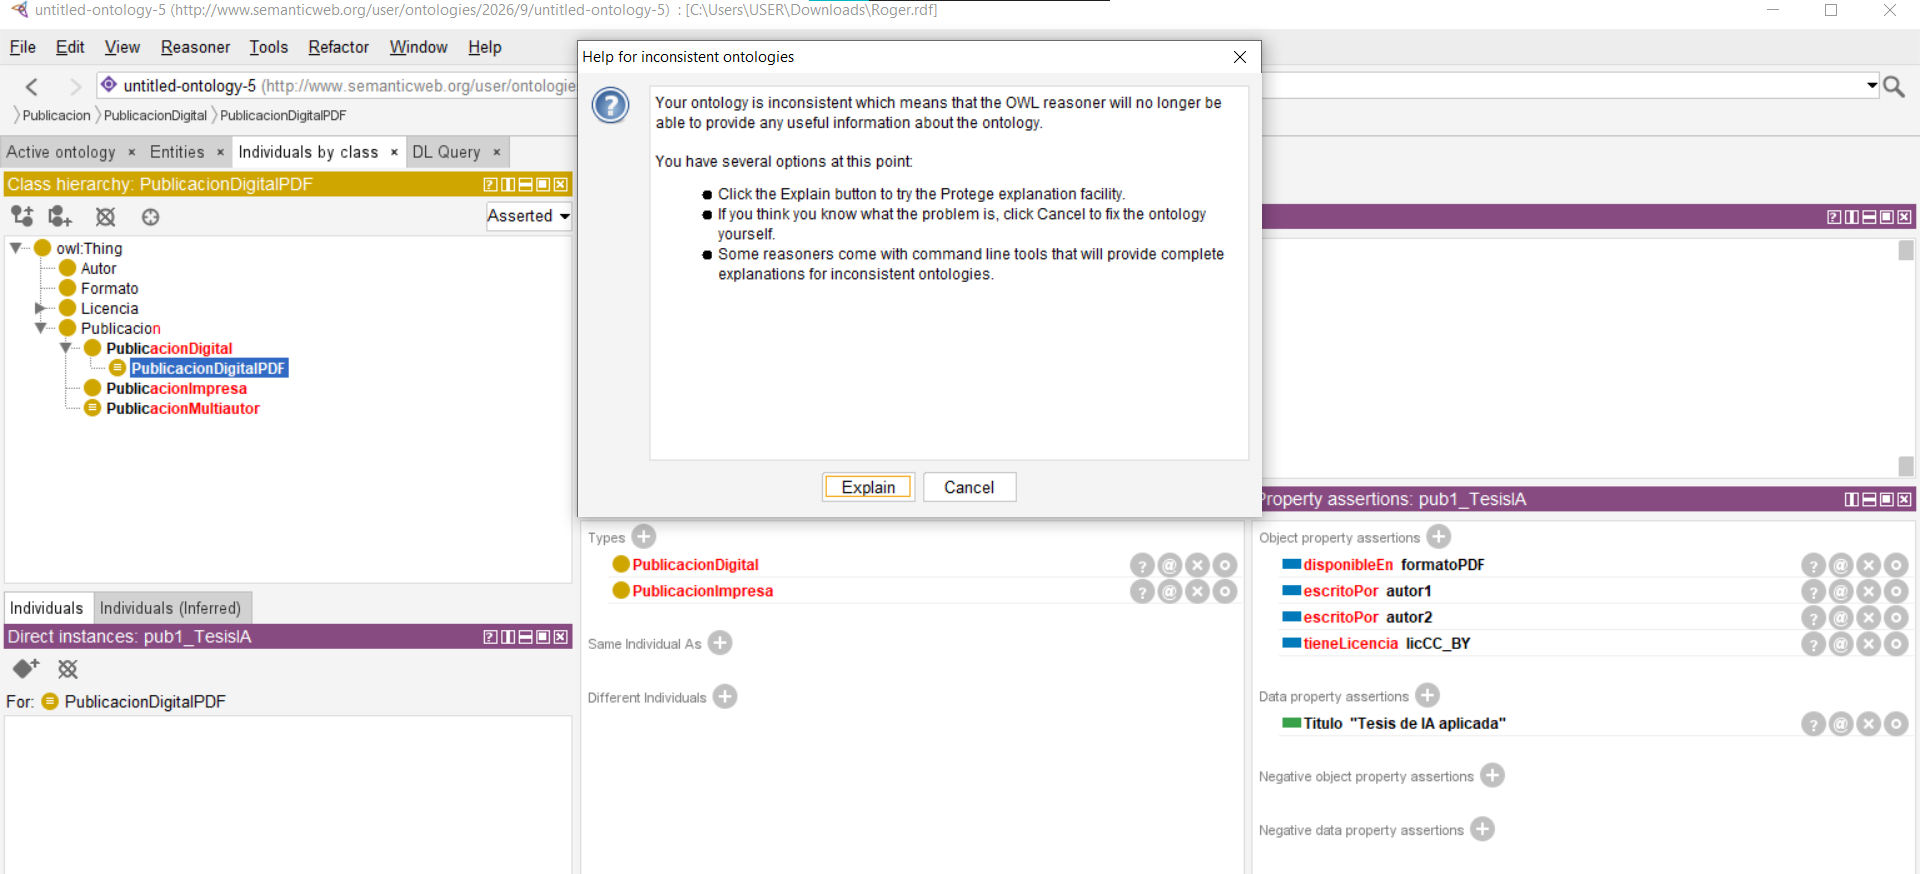
\includegraphics[width=0.86\linewidth,height=\textheight,keepaspectratio]{capturas/p4_31.png}\}

La ventana previa declara que la ontología no es consistente

Mostrando justificación lógica

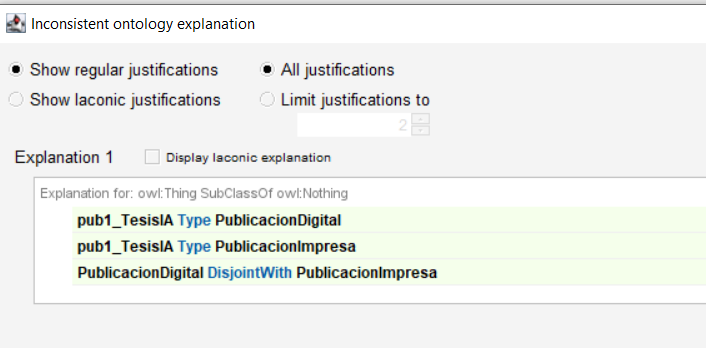
\includegraphics[width=0.86\linewidth,height=\textheight,keepaspectratio]{capturas/p4_32.png}\}

Este cuadro explica que PublicacionDigital y PublicacionImpresa son
disjuntas.

\subsection{Lectura de resultados (inferencias esperadas y por qué se
producen)}\label{lectura-de-resultados-inferencias-esperadas-y-por-quuxe9-se-producen}

Antes de ejecutar HermiT se esperaba:

{\def\LTcaptype{none} % do not increment counter
\begin{longtable}[]{@{}
  >{\raggedright\arraybackslash}p{(\linewidth - 4\tabcolsep) * \real{0.3333}}
  >{\raggedright\arraybackslash}p{(\linewidth - 4\tabcolsep) * \real{0.3333}}
  >{\raggedright\arraybackslash}p{(\linewidth - 4\tabcolsep) * \real{0.3333}}@{}}
\toprule\noalign{}
\begin{minipage}[b]{\linewidth}\raggedright
\#
\end{minipage} & \begin{minipage}[b]{\linewidth}\raggedright
Inferencia esperada
\end{minipage} & \begin{minipage}[b]{\linewidth}\raggedright
Condición que la permite
\end{minipage} \\
\midrule\noalign{}
\endhead
\bottomrule\noalign{}
\endlastfoot
1 & \texttt{pub1\_TesisIA} es \texttt{PublicacionMultiautor} & Tiene 2
autores (\texttt{autor1}, \texttt{autor2}) declarados distintos
(\texttt{DifferentIndividuals}) → cumple
\texttt{escritoPor\ min\ 2\ Autor}. \\
2 & \texttt{pub1\_TesisIA} es \texttt{PublicacionDigitalPDF} & Es
\texttt{PublicacionDigital} y \texttt{disponibleEn\ formatoPDF} → cumple
la equivalencia con \texttt{hasValue\ formatoPDF}. \\
\end{longtable}
}

HermiT confirma ambas: en la vista de \texttt{pub1\_TesisIA} aparecen en
amarillo los tipos inferidos \texttt{PublicacionDigitalPDF} y
\texttt{PublicacionMultiautor}. La inferencia 1 se produce por la clase
definida con cardinalidad mínima (\texttt{min\ 2}) combinada con
individuos distintos (sin \texttt{DifferentIndividuals}, el razonador
podría fusionar \texttt{autor1} y \texttt{autor2} y no dispararía). La
inferencia 2 se produce por la clase definida con
\texttt{hasValue\ formatoPDF} sobre una publicación digital.

\subsection{d) Prueba de incompatibilidad
(explicación)}\label{d-prueba-de-incompatibilidad-explicaciuxf3n}

Al asignar a un individuo dos clases declaradas disjuntas
(\texttt{PublicacionDigital} y \texttt{PublicacionImpresa}), HermiT
declara la ontología inconsistente
(\texttt{Help\ for\ inconsistent\ ontologies}) y se niega a razonar
hasta corregir el modelo. La justificación lógica muestra que ambas
clases son disjuntas, por lo que ningún individuo puede pertenecer a
ambas a la vez.
